\documentclass{article}
\usepackage{fullpage,graphicx}
\usepackage{amsmath,amsfonts,amsthm,amssymb,multirow}
\usepackage{algorithmic,comment,url}
\usepackage{tikz}
\usetikzlibrary{decorations.pathreplacing, shapes}
\usepackage[ruled,vlined,commentsnumbered,titlenotnumbered]{algorithm2e}
\newcommand{\expecting}[1]{\noindent{[\textbf{We are expecting:} \em #1\em]}}
\newcommand{\hint}[1]{\noindent{[\textbf{HINT:} \em #1 \em]}}
\newcommand{\pts}[1]{\textbf{(#1 pt.)}}


\begin{document}
\noindent
CS 161 \hfill \textbf{Problem Set 3} \newline 
{Winter 2019} \hfill \textbf{Due:} Friday, February 8, 2019, at 3pm on Gradescope

\noindent
\rule{\linewidth}{0.4pt}

\section*{Exercises}
Please do the exercises on your own.

\noindent
\rule{\linewidth}{0.4pt}
\begin{enumerate}

\item \pts{2} For each of the following examples, if the nodes can be colored red or black to make a legitimate red-black tree, then give such a coloring.  If not, then say that they cannot.  

(For reference, the \LaTeX code to make these trees is included at the end of the PSET, as well as instructions about how to color the nodes red or black.  If you use this code, make sure you include \verb|\usepackage{tikz}| before the \verb|\begin{document}| command.   You are also welcome to take a screenshot and color the trees in MSPaint, or make a hand-drawn copy and take a photo, or...)

\begin{center}
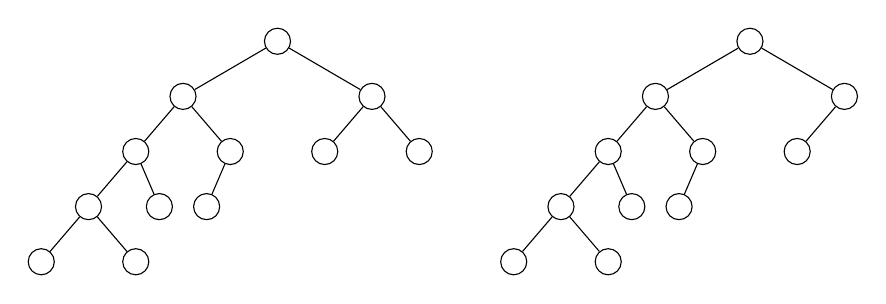
\begin{tikzpicture}[xscale=0.6,yscale=.7]
\begin{scope}
\node[draw,circle](b) at (0,0) {};
\node[draw,circle](b0) at (-2,-1) {};
\node[draw,circle](b1) at (2,-1) {};
\node[draw,circle](b00) at (-3,-2) {};
\node[draw,circle](b01) at (-1,-2) {};
\node[draw,circle](b10) at (1,-2) {};
\node[draw,circle](b11) at (3,-2) {};

\node[draw,circle](b000) at (-4,-3) {};
\node[draw,circle](b001) at (-2.5,-3) {};
\node[draw,circle](b010) at (-1.5,-3) {};

\node[draw,circle](b0000) at (-5,-4) {};
\node[draw,circle](b0001) at (-3,-4) {};

\draw (b) -- (b0);
\draw (b) -- (b1);
\draw (b0) -- (b00);
\draw (b0) -- (b01);
\draw (b1) -- (b10);
\draw (b1) -- (b11);
\draw (b00) -- (b000);
\draw (b00) -- (b001);
\draw (b01) -- (b010);
\draw (b000) -- (b0000);
\draw (b000) -- (b0001);
\end{scope}

\begin{scope}[xshift=10cm]
\node[draw,circle](b) at (0,0) {};
\node[draw,circle](b0) at (-2,-1) {};
\node[draw,circle](b1) at (2,-1) {};
\node[draw,circle](b00) at (-3,-2) {};
\node[draw,circle](b01) at (-1,-2) {};
\node[draw,circle](b10) at (1,-2) {};

\node[draw,circle](b000) at (-4,-3) {};
\node[draw,circle](b001) at (-2.5,-3) {};
\node[draw,circle](b010) at (-1.5,-3) {};

\node[draw,circle](b0000) at (-5,-4) {};
\node[draw,circle](b0001) at (-3,-4) {};

\draw (b) -- (b0);
\draw (b) -- (b1);
\draw (b0) -- (b00);
\draw (b0) -- (b01);
\draw (b1) -- (b10);
\draw (b00) -- (b000);
\draw (b00) -- (b001);
\draw (b01) -- (b010);
\draw (b000) -- (b0000);
\draw (b000) -- (b0001);

\end{scope}
\end{tikzpicture}
\end{center}

\expecting{For each tree, either an image of a colored-in red-black tree or a statement ``No such red-black tree.''  No justification is required.}

%%%%%%%%%%%%%%%%%%%

\item \pts{6} In this exercise, we'll explore different types of randomized algorithms.  We say that a randomized algorithm is a \textbf{Las Vegas algorithm} if it is always correct (that is, whenever it returns, it returns the right answer), but the running time is a random variable.  We say that a randomized algorithm is a \textbf{Monte Carlo algorithm} if there is some probability that it is incorrect.  For example, QuickSort (with a random pivot) is a Las Vegas algorithm, since it always returns a sorted array, but it might be slow if we get very unlucky.

The penguin population from PSET 2 is back, and you want to solve the same problem as you did on PSET 2 using randomized algorithms.  
As a reminder, there are $n$ penguins on an island, of many different species.  You can't tell the penguins apart, but there's an expert penguinologist who can, and she can answer queries to \texttt{isTheSame(p1,p2)} which returns True if \texttt{p1} and \texttt{p2} are penguins of the same species, and False otherwise.  Your goal is to find a member of the majority species (assuming there is one).  Consider the three algorithms seen in Figure~\ref{algs}, all of which call the subroutine \textsc{isMajority} (also seen in Figure~\ref{algs}), and all of which attempt to find a majority penguin.

\begin{figure}%[h!]

\begin{algorithm}[H]
\KwIn{A population $P$ of $n$ penguins}
\While{true}
{
Choose a random $p \in P$\; 
\If{\textsc{isMajority}($P,p$)}{ \Return{ $p$}\; }
}
\caption{\textsc{findMajorityPenguin1}}
\end{algorithm}

\begin{algorithm}[H]
\KwIn{A population $P$ of $n$ penguins}
\For{100 iterations}
{
Choose a random $p \in P$\;
\If{\textsc{isMajority}($P,p$)}{ \Return{ $p$ }\;}
}
\Return{ $P[0]$\;}
\caption{\textsc{findMajorityPenguin2}}
\end{algorithm}

\begin{algorithm}[H]
\KwIn{A population $P$ of $n$ penguins}
Put the penguins in $P$ in a random order.\;

\tcc{Assume it takes time $\Theta(n)$ to put the $n$ penguins in a random order}
\For{ $p \in P$ }
{
\If{\textsc{isMajority}($P,p$)}{ \Return{ $p$ }\; }
}
\caption{\textsc{findMajorityPenguin3}}
\end{algorithm}

\begin{algorithm}[H]
\KwIn{A population $P$ of $n$ penguins and a penguin $p \in P$}
\KwOut{True if $p$ is a member of a majority species}

count $\gets$ 0\;
\For{ $q \in P$ }
{
	\If{ \textsc{isTheSame}($p$,$q$) }{ count ++\;}
}
\If{ count $> n/2$ }{\Return{True}\;}
\Else{\Return{False}\;}
\caption{\textsc{isMajority}}
\end{algorithm} 

\caption{Three randomized algorithms for finding a majority penguin}\label{algs}

\end{figure}

Fill in the table below, and justify your answers.
If it is helpful, the \LaTeX code for the table is copied at the end of the problem set.

\begin{center}
\begin{tabular}{|c|p{3cm}|p{2cm}|p{2cm}|p{4cm}|}
\hline
Algorithm & Monte Carlo or Las Vegas? & Expected running time 
& Worst-case running time & Probability of returning a majority penguin \\
\hline
\textbf{Algorithm 1} &  &  &  & \\
\hline
\textbf{Algorithm 2} &  &  &  & \\
\hline
\textbf{Algorithm 3} &  &  &  & \\
\hline
\end{tabular}
\end{center}

\expecting{Your filled in-table, and a short justification for each entry of the table.
You may use asymptotic notation for the running times; for the probability of returning a majority penguin, give the tightest bound that you can given the information provided.
}

%%%%%%%%%%

\newpage
\item\pts{3} This exercise references the IPython notebook \texttt{HW3.ipynb}, available on the course website.  

In our implementation of radixSort in class, we used bucketSort to sort each digit.  Why did we use bucketSort and not some other sorting algorithm?  There are several reasons,  and we'll explore one of them in this exercise.

\begin{enumerate}
\item\pts{1} One reason we chose bucketSort was that it makes radixSort work correctly!  In \texttt{HW3.ipynb}, we've implemented four different sorting algorithms---bucketSort, quickSort, and two versions of mergeSort---as well as radixSort.  

\textbf{Note:} The IPython notebook is long, but just because it implements many different sorting algorithms.  Don't get scared!  

There is a \texttt{TODO} statement in the IPython notebook where you can change the code to use different sorting algorithms; you just have to make sure that the sorting algorithm you want to use is the one that is not commented out.
Modify the code for radixSort to use each one of these four algorithms within radixSort, and test it out on the examples suggested.

Which sorting algorithms seem to be correct as ``inner sorting algorithms'' for radixSort? 
\begin{enumerate}
	\item Does using bucketSort always work correctly?
	\item Does using quickSort always work correctly?
	\item Does using mergeSort (with merge1) always work correctly?
	\item Does using mergeSort (with merge2) always work correctly?
\end{enumerate}
\expecting{Yes or no for each part.}
\item\pts{2} Explain what you saw above.  What was special about the algorithms which worked?  Why does this special thing matter?  (You may wish to play around with \texttt{HW3.ipynb} to ``debug" the incorrect cases.)

\expecting{A clear definition of the special property that the correct algorithms have, and a few sentences explaining why it matters.
You do not need to justify 
why each of the algorithms do or do not have the property.}

\end{enumerate}

%%%%%%%%%%%%


\end{enumerate}
\newpage
\noindent
\rule{\linewidth}{0.4pt}
\section*{Problems}
You may talk with your fellow CS161-ers about the problems.  However:
\begin{itemize}
	\item Try the problems on your own \em before \em collaborating.
	\item Write up your answers yourself, in your own words.   You should never share your typed-up solutions with your collaborators.
	\item If you collaborated, list the names of the students you collaborated with at the beginning of each problem.
\end{itemize}

\noindent
\rule{\linewidth}{0.4pt}


\begin{enumerate}
\setcounter{enumi}{3}

\item \pts{6} [\textbf{Duck.}] Suppose that $n$ ducks are standing in a line.  
\begin{center}
\includegraphics[width=1cm]{duck}
\hspace{1cm}
\includegraphics[width=1cm]{duck}
\hspace{1cm}
\includegraphics[width=1cm]{duck}
\hspace{1cm}
\includegraphics[width=1cm]{duck}
\hspace{1cm}
\includegraphics[width=1cm]{duck}
\hspace{1cm}
\includegraphics[width=1cm]{duck}
\end{center}

Each duck has a political leaning: left, right, or center.  You'd like to sort the ducks so that all the left-leaning ones are on the left, the right-leaning ones are on the right, and the centrist ducks are in the middle.
You can only do two sorts of operations on the ducks:

\begin{center}
\begin{tabular}{|c|c|c|}
\hline
Operation & Result\\
\hline
\texttt{poll(j)} & Ask the duck in position $j$ about its political leanings \\ 
\hline
\texttt{swap(i,j)} & Swap the duck in position $j$ with the duck in position $i$ \\
\hline
\end{tabular}
\end{center}

However, in order to do either operation, you need to pay the ducks to co-operate: each operation costs one stale hot dog bun.\footnote{Probably you shouldn't be feeding ducks stale hot dog buns, but that's all you have.}  Also, you didn't bring a piece of paper or a pencil, so you can't write anything down and have to rely on your memory.  Like many humans, you can remember up to seven\footnote{see, e.g., \url{https://en.wikipedia.org/wiki/The_Magical_Number_Seven,_Plus_or_Minus_Two}} integers between $0$ and $n-1$ at a time.

\begin{enumerate}
\item \pts{4}
Design an algorithm to sort the ducks which costs $O(n)$ stale hot dog buns, and uses no extra memory other than storing at most seven\footnote{You don't need to use all seven storage spots, but you can if you want to.  Can you do it with only two?} integers between $0$ and $n$.

\expecting{Pseudocode \textbf{AND} a short English description of your algorithm.}

\item \pts{2} Justify why your algorithm is correct, and why it uses only $O(n)$ stale hot dog buns and stores at most seven integers at a time. 

\expecting{An informal justification which is both clear and convincing to the grader.  If it's easier for you to be clear, you can give a formal proof of correctness, but you do not have~to.}
\end{enumerate}

%%%%%%%%%%%%%

\newpage
\item \pts{5} [\textbf{Duck.}] Suppose that $n$ ducks are standing in a line, ordered from shortest to tallest.
\begin{center}
\includegraphics[height=1.8cm]{yardstick}
\includegraphics[width=1cm,height=1cm]{duck}
\hspace{1cm}
\includegraphics[width=1cm,height=1.4cm]{duck}
\hspace{1cm}
\includegraphics[width=1cm,height=1.6cm]{duck}
\hspace{1cm}
\includegraphics[width=1cm,height=1.9cm]{duck}
\hspace{1cm}
\includegraphics[width=1cm,height=2cm]{duck}
\hspace{1cm}
\includegraphics[width=1cm,height=2.5cm]{duck}
\end{center}

You have a measuring stick of a certain height, and you would like to identify duck which is the same height as the stick, or else report that there is no such duck.  The only operation you are allowed to do is \texttt{compareToStick(j)}, where $j \in \{0,\ldots, n-1\}$, which returns \texttt{taller} if the $j$'th duck is taller than the stick, \texttt{shorter} if the $j$'th duck is shorter than the stick, and \texttt{the same} if the $j$'th duck is the same height as the stick.  As in Problem 4, 
%you forgot to bring a piece of paper, so you can only store up to seven integers in $\{0,\ldots,n\}$ at a time.  And, as in Problem 4,  %% We removed this requirement!
you have to pay a duck one stale hot dog bun in order to compare it to the stick.

\begin{enumerate}
\item \pts{2} Give an algorithm which either finds a duck the same height as the stick, or else returns ``No such duck," in the model above which uses $O(\log(n))$ stale hot dog buns.

\expecting{Pseudocode \textbf{AND} an English description of your algorithm.  You do not need to justify the correctness or stale hot dog bun usage. } 
\item \pts{3} Prove that any algorithm in this model of computation must use $\Omega(\log(n))$ stale hot dog buns.

\expecting{A short but convincing argument.}
\end{enumerate}

%%%%%%%%%%%%%%

\item \pts{4} [\textbf{Goose!}]  A goose comes to you with the following claim.  They say that they have come up with a new kind of binary search tree, called \texttt{gooseTree}, even better than red-black trees!

More precisely, \texttt{gooseTree} is a data structure that stores data in a binary search tree.  It might also store other auxiliary information, but the goose won't tell you how it works.  The goose claims that \texttt{gooseTree} supports the following operations:
\begin{itemize}
\item \texttt{gooseInsert(k)} inserts an item with key $k$ into the \texttt{gooseTree}, maintaining the BST property.  It does not return anything.  It runs in time $O(1)$.
\item \texttt{gooseSearch(k)} finds and returns a pointer to node with key $k$, if it exists in the tree.  It runs in time $O(\log(n))$, where $n$ is the number of items in the \texttt{gooseTree}.
\item \texttt{gooseDelete(k)} removes and returns a pointer to an item with key $k$, if it exists in the tree, maintaining the BST property.  It runs in time $O(\log(n))$, where $n$ is the number of items in the \texttt{gooseTree}.
\end{itemize}
The goose says that all these operations are deterministic, and that \texttt{gooseTree} can handle arbitrary comparable objects.

You think the goose's logic is a bit loosey-goosey.  How do you know the goose is wrong?

\expecting{A formal proof that the goose must be wrong.  (It is okay if it is a short proof).  You may use results or algorithms that we have seen in class without further justification.} 


\hint{Since the goose won't tell you how \texttt{gooseTree} works, you cannot assume anything about how \texttt{gooseInsert}, \texttt{gooseSearch} or \texttt{gooseDelete} might be implemented.}

\hint{Because \texttt{gooseTree} stores a BST, you can still do \texttt{inOrderTraversal} in time $O(n)$.}

%%%%%%%%%%%%%%%%

\end{enumerate}
\newpage
\section*{Feedback}
This part is not worth any points, but it is quick, painless, and anonymous, and we'd really appreciate it if you help us out by giving us feedback!

\begin{enumerate}
\item \pts{0} Please fill out the following poll, which asks your opinion on the homework:
\begin{center}
\url{https://goo.gl/forms/eSssHWRPgRUva6bA2}
\end{center}
\end{enumerate}
\newpage
\section*{Helpful \LaTeX code!}
Here is some code to generate the red-black trees; we've shown how to color one of the nodes green, you can use this example to color them red or black.  You are also welcome to take a screenshot and color in your favorite paint program, or include a picture of a hand-drawn image, or any other way you can think of getting a picture of a colored red-black tree into your PSET.
\footnotesize
\begin{verbatim}
\begin{center}
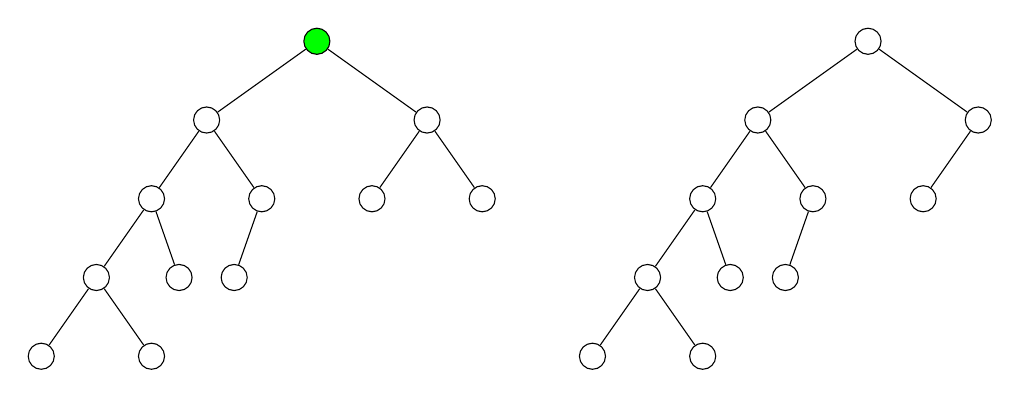
\begin{tikzpicture}[xscale=0.7]
\begin{scope}
\node[draw,circle,fill=green](b) at (0,0) {};
\node[draw,circle](b0) at (-2,-1) {};
\node[draw,circle](b1) at (2,-1) {};
\node[draw,circle](b00) at (-3,-2) {};
\node[draw,circle](b01) at (-1,-2) {};
\node[draw,circle](b10) at (1,-2) {};
\node[draw,circle](b11) at (3,-2) {};
\node[draw,circle](b000) at (-4,-3) {};
\node[draw,circle](b001) at (-2.5,-3) {};
\node[draw,circle](b010) at (-1.5,-3) {};
\node[draw,circle](b0000) at (-5,-4) {};
\node[draw,circle](b0001) at (-3,-4) {};
\draw (b) -- (b0);
\draw (b) -- (b1);
\draw (b0) -- (b00);
\draw (b0) -- (b01);
\draw (b1) -- (b10);
\draw (b1) -- (b11);
\draw (b00) -- (b000);
\draw (b00) -- (b001);
\draw (b01) -- (b010);
\draw (b000) -- (b0000);
\draw (b000) -- (b0001);
\end{scope}

\begin{scope}[xshift=10cm]
\node[draw,circle](b) at (0,0) {};
\node[draw,circle](b0) at (-2,-1) {};
\node[draw,circle](b1) at (2,-1) {};
\node[draw,circle](b00) at (-3,-2) {};
\node[draw,circle](b01) at (-1,-2) {};
\node[draw,circle](b10) at (1,-2) {};
\node[draw,circle](b000) at (-4,-3) {};
\node[draw,circle](b001) at (-2.5,-3) {};
\node[draw,circle](b010) at (-1.5,-3) {};
\node[draw,circle](b0000) at (-5,-4) {};
\node[draw,circle](b0001) at (-3,-4) {};
\draw (b) -- (b0);
\draw (b) -- (b1);
\draw (b0) -- (b00);
\draw (b0) -- (b01);
\draw (b1) -- (b10);
\draw (b00) -- (b000);
\draw (b00) -- (b001);
\draw (b01) -- (b010);
\draw (b000) -- (b0000);
\draw (b000) -- (b0001);
\end{scope}

\end{tikzpicture}
\end{center}
\end{verbatim}
\newpage
\normalsize
Here is the code that generated the table for the penguin exercise:

\begin{verbatim}
\begin{center}
\begin{tabular}{|c|p{3cm}|p{2cm}|p{2cm}|p{4cm}|}
\hline
Algorithm & Monte Carlo or Las Vegas? & Expected running time 
& Worst-case running time & Probability of returning a majority penguin \\
\hline
\textbf{Algorithm 1} &  &  &  & \\
\hline
\textbf{Algorithm 2} &  &  &  & \\
\hline
\textbf{Algorithm 3} &  &  &  & \\
\hline
\end{tabular}
\end{center}
\end{verbatim}

\end{document}
